\documentclass[12pt, a4paper, oneside]{ctexart}

\usepackage[table]{xcolor}

\usepackage{graphicx,amsmath,amssymb,geometry,float}

\usepackage{listings}
\usepackage{matlab-prettifier}

\usepackage{enumerate,enumitem}
\usepackage{autobreak}
\usepackage{breqn}

\geometry{left=2.5cm, right=2.5cm, top=2.5cm, bottom=2.5cm}

\usepackage{booktabs,array,tabularx}

\usepackage{fancyhdr}
\renewcommand{\footrulewidth}{0.4pt}
\renewcommand{\headrulewidth}{0.4pt}
\pagestyle{fancy}
\fancyhf{}
\cfoot{\thepage}


\newtheorem{assumption}{假设}[section]

\CTEXsetup[name={,、\hspace{-1em}},number={\chinese{section}}]{section}






\begin{document}
\begin{abstract}

\end{abstract}
\newpage
\section{问题重述}
\subsection{问题背景}
如今,化石燃料和环境保护已成为世界上最热门的问题。世界范围内的主要交通工具以石油为主,造成了严重的环境污染。由于化石燃料的资源有限,而且总是导致污染,因此向更清洁的能源过渡是不可避免的。为了实现这一目标,以新能源汽车为代表的电动汽车被公认为21世纪汽车产业转型的主要发展方向。

众所周知,电动汽车效率高、噪音低、污染几乎为零。电动汽车的优势显而易见。因此,它们已在世界各地广泛使用。推动电动汽车的规模化发展,需要完善相应的基础设施。充电站作为电动汽车设施建设的重要组成部分,对整个电动汽车产业的发展至关重要。我们需要在哪里和多少个充电站建设?选择正确的位置和估计充电站的数量非常重要。

随着温室效应和空气污染问题的加剧,各国都在寻找新能源来替代传统燃料,如原油或柴油,以缓解日益严重的空气问题。自混合动力汽车和燃气汽车问世以来,新型清洁汽车的探索仍在不断进行。目前,以特斯拉为首的电动汽车将在更大程度上突破能源和经济的限制,更好地平衡快速增长的汽车需求与环境的关系。充电站数量合适,距离合适,对于电动汽车的普及至关重要。与加油站相比,电动汽车充电站占用的空间更小,具有更高的安全系数,可以更好地分布在街道和社区,让人们更方便、更高效地使用。然而,电动汽车的推广并非一蹴而就。要逐步扩大电动汽车覆盖面,不断完善电动汽车充电站网络,最终完成汽油和柴油汽车的终结运营。另外,不同国家的经济、文化条件不同,需要根据自己的具体情况确定推广时间和推广范围,才能取得更好的效果。要逐步扩大电动汽车覆盖面,不断完善电动汽车充电站网络,最终完成汽油和柴油汽车的。
\subsection{具体问题重述}
\subsubsection{第一问}
开发一算法来确定某地区的充电站系统,包括充电站的位置和数量,并预测未来增长情况。

\subsubsection{第二问}
根据开发的算法进行结果的分析和讨论,找出未来影响电动汽车发展战略的主要因素,预测电动汽车未来发展的趋势。

\section{问题分析}

\section{符号说明}
\begin{table}[H]
    \caption{符号说明}
    \centering
    \renewcommand{\arraystretch}{2}
    \begin{tabular*}{\textwidth}{c||l}%l左对齐,c居中,r右对齐,p指定列宽度
        \toprule[1.5mm]
        \Large{\textbf{符号}} & \Large{\textbf{说明}} \\
        \midrule[1.5pt]
        \(d_{ij}\) & OD距离成本矩阵,表示i地到j地的距离 \\\hline
        \(q_i\)&需求列表,表示i地的车辆数量(即对充电桩的需求量)\\\hline
        \(p\)&总充电桩数量\\\hline
        \(n_i\)&供应列表,表示i地安装的慢充充电桩数量\\\hline
        \(\rho_{ij}\)&分配矩阵,表示i地的需求以\(\rho_{ij}\)的比例分配给j地的慢充充电桩\\\hline
        \(c_j\)&容量列表,表示i地能够供应的容量,等于i地建设的慢充充电桩数量\\\hline
        \(E_k\)&续航里程\\\hline
        \(L\)&年平均行驶里程\\\hline
        \(F_k\)&百公里耗电\\\hline
        \(I\)&服务强度\\\hline
        \bottomrule[1mm]
    \end{tabular*}
\end{table}
\section{基本假设}
\begin{assumption}\label{asmp:lcpark}
    每个目的地的停车场数量足以供应目的地的车流量(无需在目的地建造新的停车场)
\end{assumption}
\begin{assumption}\label{asmp:lcload}
    慢充不会对电网产生高峰期的负荷,只需算总耗电。\\
    原因:慢充总可以智能选择一天当中电网负荷低的时候充电。
\end{assumption}
\begin{assumption}\label{asmp:lcoccupy}
    只有电量低于10\%的电动车会占用慢充车位充电并且错开(即不会所有车同时电量低于10\%),所以慢充不考虑排队只考虑总耗电;同时每天分为白天和晚上两个充电时期。
\end{assumption}
\begin{assumption}\label{asmp:cost}
    所有道路都完全相同,不存在坡度等因素会增加在道路上行驶同等距离时的耗电量。\\
    原因:首先,所有道路导致的耗电量增加可以叠加到道路的距离成本中去。其次,坡度等数据网上没有,需要对实地进行测绘等工作,在短暂的时间内无法完成。
\end{assumption}
\begin{assumption}
    \label{asmp:serve}
    车辆到达快充充电站接受服务的间隔以及服务时间的分布符合泊松分布。
\end{assumption}
\begin{assumption}
    所有长途旅行的车辆可以且最多可以在充电站排队等待1个小时。
\end{assumption}


\section{模型建立}
\subsection{充电桩选址模型}
\subsubsection{充电桩分类}
我们将充电站分为两种,分别是短时停靠充电站(简称快充,sc)和长时停靠充点站(简称慢充,lc)

长时停靠充电站用于在人们长时间停车(平均超过5h,用普通功率,车可以充满),

短时停靠充电站用于在人们长途旅行时临时充电(起到类似于加油站的作用,需在半小时内充满一辆汽车)
\subsubsection{建模前的准备:约束条件以及概念}
\begin{enumerate}[label = \roman*)]
    \item \textbf{成本}\\
          快充成本为地价和充电桩费用的叠加
          \begin{align}\begin{autobreak}
                  f_{sc}=\sum\limits_{i}(f_{ci}\cdot S_0+f_{li})\cdot n_i
              \end{autobreak}\end{align}



          慢充建在停车场,价格远低于快充且单价固定,所以对成本的限制转化为对数量的限制
          \begin{align}\begin{autobreak}
                  f_{lc}\propto p
              \end{autobreak}\end{align}
    \item \textbf{区域总耗电量q}\\
          汽车的日均总耗电量q可由如下公式计算得到:
          \begin{align}\begin{autobreak}
                  q=\frac{L}{365}\cdot \frac{F_k}{100}\cdot Po\cdot V_p\cdot \alpha_e
              \end{autobreak}\end{align}
          其中L为年平均行驶里程,\(F_k\)为百公里耗电,\(Po\)为地区人口,\(V_p\)为地区人均私家车数量,\(\alpha_e\)为电动车占比,可由电动车发展模型得到。以上数据均可以从互联网中查得。
    \item \textbf{OD距离矩阵d\(_{ij}\)}\\
          距离矩阵可以通过道路实际位置和道路拓扑结构通过对每两个节点求最短路径算出。道路数据从互联网上查得。
    \item \textbf{电网负荷Ld\(_a\)}\\
          由于中国电网很强大,且现在电动车数量稀少,我们初步模型暂时不考虑这个条件作为约束,但可以根据结果计算对电网造成的负荷。计算方法如下:\\
          慢充考虑一整天的负荷\(Ld_{lc}=\beta q/24\),\(\beta\)为损耗系数。除以24得到平均每小时负荷\\
          快充考虑高峰时期不间断充电造成的负荷:\(Ld_{sc}=P_{sc}=F_k\cdot E_k/t_{sc}\),其中\(E_k\)为续航里程,\(t_{sc}\)为快充充满所需时间。以上数据均可以从互联网中查得。

    \item \textbf{单位承载力c\(_0\)}\\
          单个充电桩所能够承载几辆车充电。我们默认\(c_0=1\)。
    \item \textbf{单次充电跨越时间T}\\
          依据假设\ref{asmp:lcoccupy},电动车从满电到10\%电量跨越的半天数\begin{align}\begin{autobreak}
                  T=\left\lfloor 0.9\frac{E_k}{L/(2\cdot 365)}\right\rfloor
              \end{autobreak}\end{align}
    \item \textbf{各节点充电桩数量n\(_i\)}\\
          各个节点充电桩数量总和应当等于充电桩总数:\(\sum\limits_i n_i=p \)
    \item \textbf{各节点需求q\(_i\)}\\
          每个节点的需求即每个节点在每个半天的所有需要充电(即电量低于10\%)的车的数量\begin{align}\begin{autobreak}
                  q_i=Po_i\cdot V_p\cdot\alpha_e/T
              \end{autobreak}\end{align}
    \item \textbf{分配矩阵\(\boldsymbol{\rho}_{ij}\)}\\
          代表i地的需求中\(\rho_{ij}\)的比例由j地满足,因此有\(\sum\limits_j \rho_{ij}=1\),即总体上每个地区的需求量被100\%地满足
    \item \textbf{道路流量F\(_i\)}\\
          每条道路的每小时流量。
    \item \textbf{排队时间W\(_s\)}\\
          指一个顾客在系统中的全部停留时间 为 期望值,记为\(W_s\),它是等待时间和服务时间的总和\(W_s=W_q+E\)。
    \item \textbf{充电桩总数p}\\
          充电桩所需的总数p可以通过总需求加上比例为\(\beta\)的冗余求得:
          \begin{equation}
              p=(1+\beta)\cdot\sum_i q_i=(1+\beta)\cdot Po\cdot V_p\cdot\alpha_e/T
          \end{equation}
          其中Po为当地人口总量。
    \item \textbf{快充站的服务模型}
    
        根据假设\ref{asmp:serve},我们选择用M/M/n的服务系统模型估计等待时间。

        首先,我们根据各个站的充电桩的数量\(n_i\)、单位时间前来充电的车数期望
        \begin{equation}
            \lambda_i=\sum\limits_j(\rho_{ji}\cdot F_j)
        \end{equation}
        以及单位时间能够充好离开的车数期望\(\mu\)可以求解出每个站服务强度
        \begin{equation}
            I_i=\frac{\lambda_i}{n_i\mu}=\frac{\sum\limits_j(\rho_{ji}\cdot F_j)}{n_i\mu}
        \end{equation}
        因此服务请求队列为k的概率,即车辆等待k-n辆即可充电的概率:
        \begin{equation*}
            p_{k}=\begin{cases}
                p_{0} \frac{I^{k}}{k !}, &1 \leqslant k<n \\
                p_{0} \frac{I^{k}}{n ! n^{k-n}}, &k \geqslant n
            \end{cases},
        \end{equation*}
        其中,
        \begin{equation}
            p_{0}=\left[\sum_{k=0}^{n-1} \frac{I^{k}}{k !}+\frac{I^{n}}{n !\left(1-\frac{I}{n}\right)}\right]^{-1}
        \end{equation}

        由此我们可以得到车辆排队等待的概率\(E_c(I)\)为:
        \begin{equation}
            E_{c}(I)=\sum_{k=n}^{\infty} p_{k}=\frac{\frac{I}{n}}{n !\left(1-\frac{I}{n}\right)} p_{0}
        \end{equation}
        最后得到车辆排队等待时间\(W_s\)为:
        \begin{equation}
            W_s=\frac{E_{c}(n, \rho)}{n \mu-\lambda}+\frac{1}{\mu}
        \end{equation}
\end{enumerate}


\subsubsection{目标优化模型的建立}
\textbf{对慢充选址的优化:}
\(d_{ij},\,q_i,\,p\)作为已知量,以\(n_j,\,\rho_{ij}\)为变量进行优化,为了使充电站位置便于人们停放,优化目标选为:使所有地区的需求者在停车充电以后所需要步行到达目的地的距离总和最小。因此所需优化的函数为:
\begin{dmath}
    f(\rho)=\sum_i \sum_jd_{ij} q_j \rho_{ij}
\end{dmath}

因此综合上面的分析可得优化方程为:
\begin{equation}
    \begin{aligned}
         & \min  f(\rho)=\sum_i \sum_jd_{ij} q_j \rho_{ij} \\
         & \begin{cases}
            \sum\limits_i n_i\leqslant p                                     & \text{(最多有p个充电桩)} \\
            \sum\limits_j \rho_{ij}=1                               & \text{(比例系数和为1)} \\
            \sum\limits_i q_{i}\rho_{ij}\leqslant c_j=n_j \cdot c_0 & \text{(承载力限制)}
        \end{cases}
    \end{aligned}
    \label{fun:优化lc}
\end{equation}

这是一个离散的线性规划模型。

\textbf{对快充选址的优化:}某人在它们的论文里证明了对于一条路上选址的最佳地点在端点,因此我们任然选取道路交叉点作为节点。这样对于快充的选址优化方程框架上与对慢充的优化方程相同,但对成本的约束不能转化为对数量的约束而应成为优化对象:
\begin{equation}
    \begin{aligned}
        & \min  \begin{cases}
            f_{sc}=\sum\limits_{i}(f_{ci}\cdot S_0+f_{li})\cdot n_i\\
            f(\rho)=\sum_i \sum_jd_{ij} q_j \rho_{ij}
        \end{cases} \\
        & \begin{cases}
           \sum\limits_j \rho_{ij}=1    & \text{(比例系数和为1)} \\
           W_{si}\leqslant W_0=1h & \text{(等待时间限制)}\\
           dis_{ij}<0.9E_k&\text{(续航里程限制)}
       \end{cases}
    \end{aligned}
\end{equation}

但是,由于快充站的建设成本远高于慢充充电桩,所以快充只用来满足长途旅行的续航问题而不关心短程开车的充电问题(这由慢充来解决)。因此,我们认为城内(地价高)的地方不用设快充充电站,而只需要在城际公路上设置。

城际公路中,高速公路上的快充站设置可以参照服务区的设置(时间先后、地点),因为服务区的设置一般是经过大量计算的。其它道路则可以根据上面的优化方程进行计算。但由于主干道路间隔较大,为了使成本降低,我们只需用快充的捕获半径覆盖全国道路\(n\cdot \frac{\sqrt3}{4}R = S\cdot \alpha\)即可(用正六边形覆盖,\(\alpha=89.26\%\)为道路覆盖率),而每个快充站的等待时间则与其捕获半径内流量有关。等待时间的限制和流量则规定了每个快充站最少的充电桩数量。





\subsection{电动车增长模型}
后面我们通过生物种群相互竞争模型来预测未来几年的电动车与燃油车的数量关系。

\subsubsection{生物种群相互竞争模型}

当某个自然的环境中只有一种生物的群体(种群)生存时,我们常用Logistic模型来描述它的数量的演变过程,即:

\begin{dmath}
  x(t)=rx(1-\frac{x}{N})
\end{dmath}

如果一个自然环境中存在两个种群,它们之间的关系为相互竞争关系,并且数量变化服从Logistic规律。

于是我们对其中一种群甲有

\begin{dmath}
  x_1(t)=r_1x_1(1-\frac{x_1}{N_1})
\end{dmath}

这里因子(\(1-\frac{x_1}{N_1}\))反映由于甲对有限资源的消耗导致的对其自身增长的阻滞作用,$\frac{x_1}{N_1}$可理解为相对于$N_1$而言,数量为$x_1$时供养甲的食物量(设食物总量为单位量1)。

当考虑到甲乙两个种群在同一自然环境中生存时考虑到乙种群消耗统一资源对甲的增长的影响,我们的因子($1-\frac{x_1}{N_1}$)再减去一项,该项与种群乙的数量成正比,得到种群甲如下式:

\begin{dmath}x_1(t)=r_1x_1\left(1-\frac{x_1}{N_1}-\sigma_1\frac{x_2}{N_2}\right)\end{dmath}

上面$\sigma_1$
  表示单位数量的种群乙消耗的供养种群甲的食物量为单位数量甲消耗的供养甲的食物量的$\sigma_1$倍。$\sigma_2$则相反同理。

\subsubsection{本题模型建立}

回到本论文中,我们将电动汽车、燃油汽车与种群甲、乙作如下类比:

$x_1(t)$表示电动车在t时间的保有量,$x_2(t)$表示燃油车在t时间的保有量。

$r_1$、$r_2$分别表示电动车与燃油车的固有增长率。

$N_1$、$N_2$为电动车与燃油车的最大容量。

$\sigma_1$
  表示电动汽车相对于传统汽车在同等经济发展下的发展优势,$\sigma_2$
表示传统汽车对电动汽车同等经济发展下的发展优势。

首先我们假设其数量遵循Logistic规律,显然电动汽车与燃油汽车两者之间存在竞争关系,故我们利用生物种群相互竞争模型来预测未来几年的电动车与柴油车的数量关系。

得到如下方程:

\begin{dmath}
  \left\{
    \begin{aligned}
      x_1(t) & = r_1x_1(1-\frac{x_1}{N_1}-\sigma_1\frac{x_2}{N_2}) \\
      x_2(t) & = r_1x_2(1-\sigma_2\frac{x_1}{N_1}-\frac{x_2}{N_2})
    \end{aligned}
    \right.
\end{dmath}

$r_1$与$r_2$我们直接根据近年来两种汽车的增长情况求解得到,其中新能源车近年来固有增长率约为50\%(2022年中国新能源汽车行业市场前景及投资研究预测报告),燃油车近年来固有增长率约为4\%(杭州统计年鉴2021)。故取$r_1=0.5,r_2=0.04$。

$N_1$、$N_2$的确定存在不确定性,需要提前估算确定。由于电动汽车与燃油汽车的功能性基本相同,我们这里假设$N_1=N_2$。
对该值的估算方法普遍有三种,分别是直接选取最大值法、专家判断法和纯粹数学推导法。本研究采用专家判断法确定两种汽车最大保有量,根据文献(《我国到底能承载多少汽车?》------姜靖、戴慧兰),国家信息中心信息资源部主任徐长明认为,汽车保有量最高可达4.5亿辆。为了合理地预估我国个人汽车保有量极限,本论文中假设其极限占比为90\%,计算得出我国个人汽车最大保有量约为4.05亿辆。

$\sigma_1$ 与$\sigma_2$
的确定我们开创性地利用主成分分析法来得到主成分数据,以得到的主成分为自变量,汽车数量为因变量通过最小二乘法作线性回归,进而得到$\sigma_1$
  与$\sigma_2$。 方法如下。

\subsubsection{相关性分析}

通过对于以往研究电动汽车发展的论文,我们注意到影响我国电动汽车保有量变化的因素有多种,如经济因素,包括人均GDP、居民收入、经济产业结构、居民消费水平等;社会因素,包括城市人口、城市化率、失业率、拥塞成本等;环境因素,包括公路网规模、基础设施完善度等。考虑长期完整数据的可获得性,我们在这里初步选取了城市人口数、城市化水平、人均GDP、居民消费水平、公路里程、第一产业占比、第二产业占比、第三产业占比这8个代表性的影响因素进行分析。(数据大部分来源于《中国统计年鉴(2021)》\cite{cite:统计年鉴})

首先我们将以上八个因素与电动汽车保有量进行了Spearman相关系数相关性分析,得到如下相关系数热力图。(电动汽车保有量来自于《2022年中国新能源汽车行业市场前景及投资研究预测报告》\cite{cite:预测报告})

\begin{figure}[H]
  \centering
  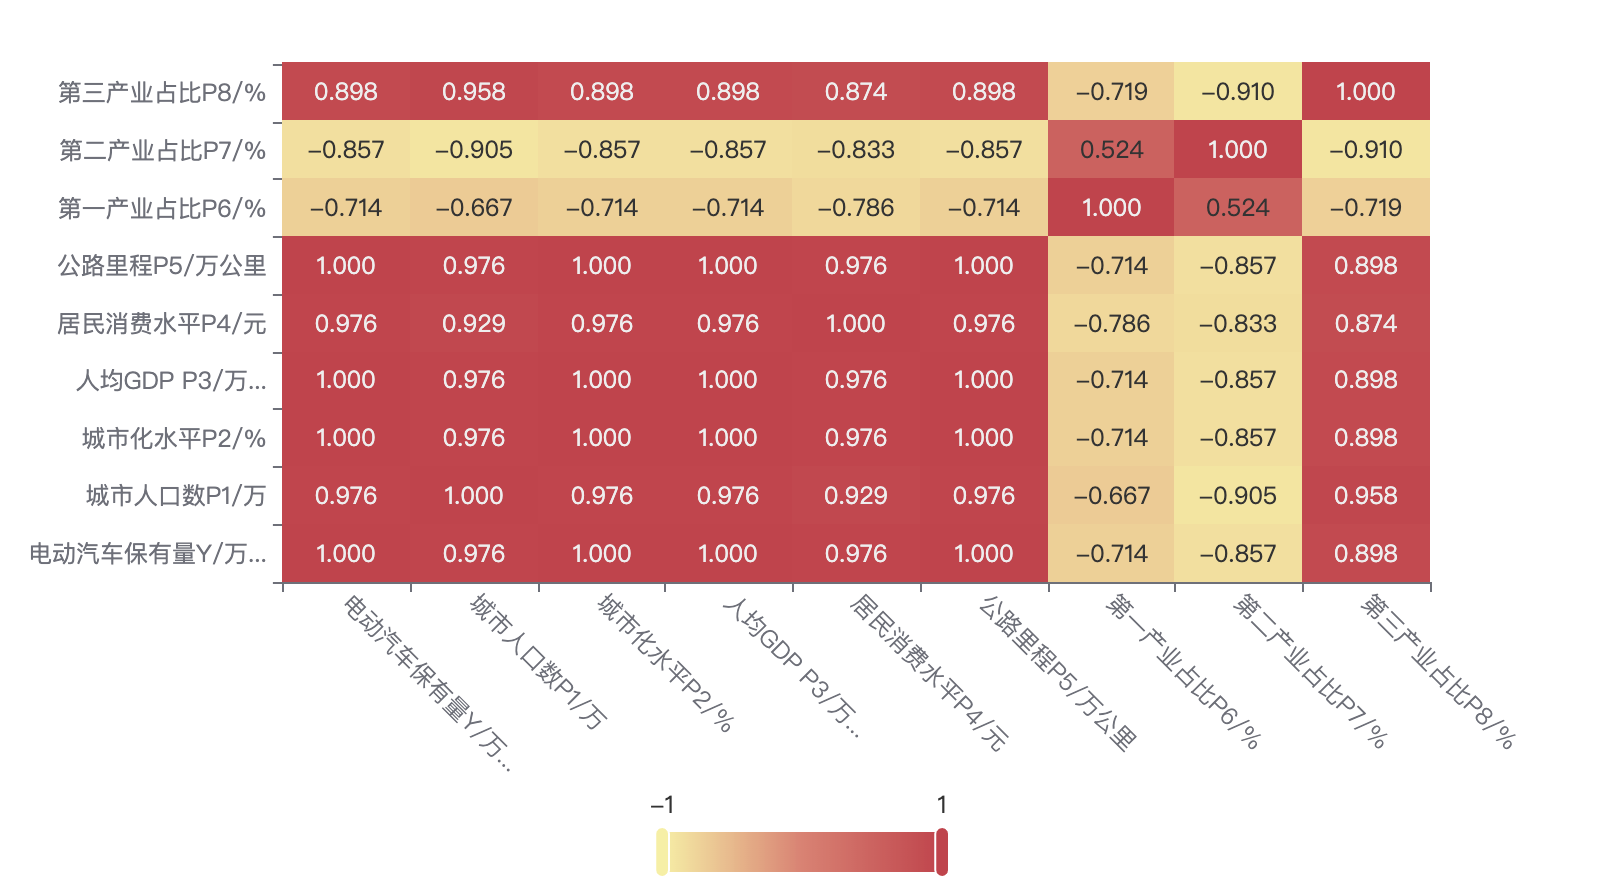
\includegraphics[width=\textwidth]{pic/相关系数热力图 (2).png}
  \caption{相关系数热力图}
  \label{fig:相关系数热力图}
\end{figure}

注意到第一产业占比、第二产业占比与电动汽车保有量相关性较低,所以我们在后续的主成分分析时略去这两种因素。

\subsubsection{{主成分分析}}

主成分分析法是运用``降维''思想,把多个指标变换成少数综合指标的多元统计方法,这里的综合指标就是主成分。每个主成分都是原始变量的线性组合,彼此相互独立,并保留了原始变量绝大部分信息。其本质是通过原始变量的相关性,寻求相关变量的综合替代对象,并且保证了转化过程中的信息损失最小
。

我们对城市人口数、城市化水平、人均GDP、居民消费水平、公路里程、第三产业占比六个因素通过SPSSPRO进行主成分分析,来综合评价每年度的社会经济发展水平。

(主成分分析的主要步骤\ldots\ldots 不知道要不要写,先省略)

KMO检验是 Kaiser, Meyer和 Olkin提出的抽样适合性检验( Measure of Sampling
Adequacy)。该检验是对原始变量之间的简相关系数和偏相关系数的相对大小进行检验。Bartlett球形度检验用于检验相关阵中各变量间的相关性,是否为单位阵,即检验各个变量是否各自独立。

我们得到KMO值=0.58,显著值p\textless0.001,水平上呈现显著性,拒绝原假设,各变量间具有相关性,主成分分析有效,效度虽然在0.6以下,但尚能接受。



\begin{table}[H]
  \centering
  \rowcolors{2}{white!20}{black!10}
  \setlength{\tabcolsep}{0.05\textwidth}{
  \begin{tabularx}{0.9\textwidth}{llXX}
    \toprule
    \rowcolor{blue!30}
    成分       & 特征根     &          &          \\
    特征根     & 方差百分比 & 累积     &          \\
    1          & 5.657      & 94.286\% & 94.286\% \\
    2          & 0.278      & 4.636\%  & 98.922\% \\
    3          & 0.056      & 0.927\%  & 99.849\% \\
    4          & 0.007      & 0.111\%  & 99.96\%  \\
    5          & 0.002      & 0.039\%  & 99.999\% \\
    6          & 0.000      & 0.001\%  & 100.0\%  \\
    \bottomrule
  \end{tabularx}}
  \caption{总方差解释}
  \label{tab:总方差}
\end{table}


\begin{figure}[H]
  \centering
  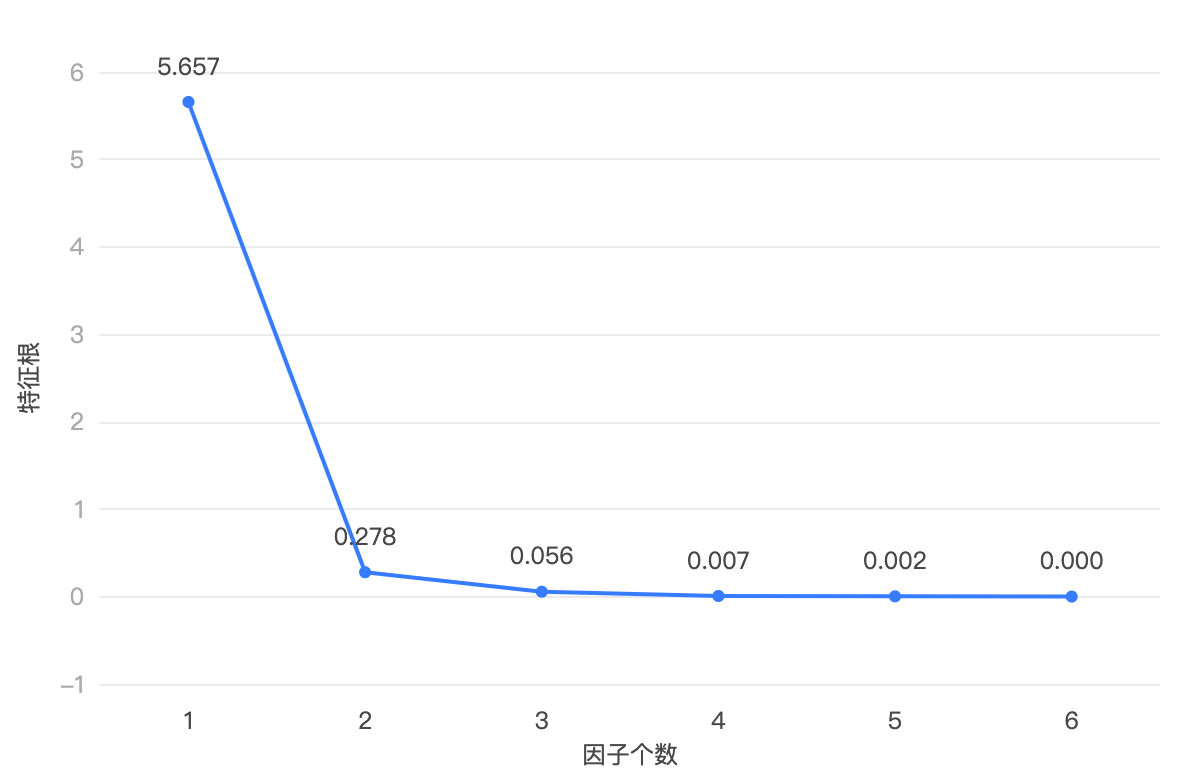
\includegraphics[width=0.8\textwidth]{pic/因子分析碎石图.png}
  \caption{因子分析碎石图}
  \label{fig:因子分析碎石图}
\end{figure}

上面方差解释表中,我们发现第一主成分的特征值λ=5.657\textgreater1,,且远大于其他特征值,
累积方差贡献率为94.286\%,
即可以解释总体数据的94.286\%。由碎石图可知,在第二个主成分开始特征值下降坡度变缓,且前两个主成分累积解释贡献率超过90\%,因此我们选择两个主成分进行分析。

从下面的因子载荷矩阵热力图中可以分析每个主成分中隐变量的重要性,其中第一个主成分与前五个因素都具有较大的相关性(0.9以上),我们概括为``城市总体发展程度''。主成分2与第三产业占比的相关程度较大,可以概括为``服务业发展程度''。

% \begin{figure}[H]
%   \centering
%   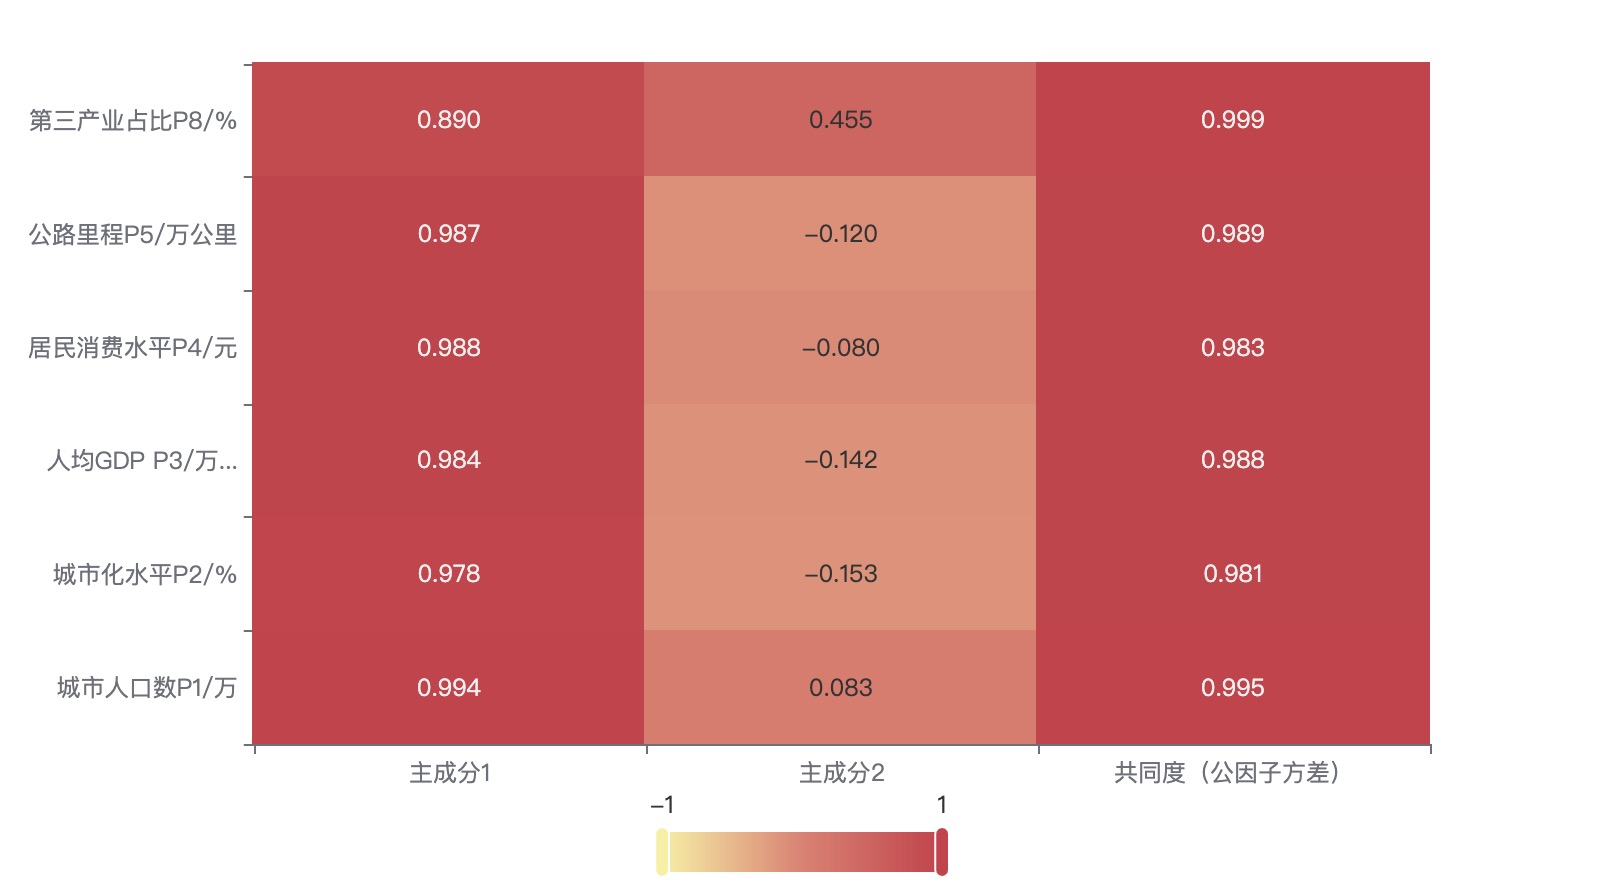
\includegraphics[width=\textwidth]{pic/相关系数热力图 (3).png}
%   \caption{相关系数热力图}
%   \label{fig:相关系数热力图3}
% \end{figure}

根据表\ref{tab:总方差}我们得到模型的公式:

\begin{dmath}
  F1=0.176\times\mbox{\bf 城市人口数}P1+0.173\times\mbox{\bf 城市化水平}P2+0.174\times\mbox{\bf 人均GDP}P3+0.175\times\mbox{\bf 居民消费水平}P4+0.174\times\mbox{\bf 公路里程}P5+0.157\times\mbox{\bf 第三产业占比}P8
\end{dmath}

\begin{dmath}
  F2=0.299\times\mbox{\bf 城市人口数}P1-0.549\times\mbox{\bf 城市化水平}P2-0.511\times\mbox{\bf 人均GDP}P3-0.289\times\mbox{\bf 居民消费水平}P4-0.433\times\mbox{\bf 公路里程}P5+1.635\times\mbox{\bf 第三产业占比}P8
\end{dmath}

由上可以得到:

\begin{dmath}
  F=(0.943/0.989)\times F1+(0.046/0.989)\times F2
\end{dmath}

\begin{table}[H]
  \centering
  \rowcolors{2}{white!20}{black!10}
  \setlength{\tabcolsep}{0.07\textwidth}{
  \begin{tabularx}{0.9\textwidth}{lXX}
    \toprule
    \rowcolor{blue!30}
      &\multicolumn{2}{c}{成分}\\
    \rowcolor{blue!30}
       \multicolumn{1}{c}{名称}  &成分1 &  成分2\\
    城市人口数P1/万   & 0.176 & 0.299  \\
    城市化水平P2/\%   & 0.173 & -0.549 \\
    人均GDP P3/万元   & 0.174 & -0.511 \\
    居民消费水平P4/元 & 0.175 & -0.289 \\
    公路里程P5/万公里 & 0.174 & -0.433 \\
    第三产业占比P8/\% & 0.157 & 1.635  \\
    \bottomrule
  \end{tabularx}}
  \caption{成分矩阵表}
  \label{tab:成分矩阵表}
\end{table}


由下图可知:第一主成分值与年份呈显著的线性正相关,
故利用线性回归模型得出第一主成分(y)与年份(x)的关系, 如式:

\begin{dmath}
  y=0.4071x-820.4
\end{dmath}

% \begin{figure}[H]
%   \centering
%   \includegraphics{https://tkoghgi47p.feishu.cn/space/api/box/stream/download/asynccode/?code=NTY2MzY4ZDViMmU5N2JmOWU0ZmE5OTgyZGVhNmFhM2NfN0xrZVdBbjVJZ2VrVHpvU1N2NmdkdDNRVlM4VWxSdE9fVG9rZW46Ym94Y25yNUhGSEpnQjNQcmZUMGJTSUtJRDJBXzE2NTI5Mzg4NjM6MTY1Mjk0MjQ2M19WNA}
%   \caption{}
% \end{figure}

第一主成分与电动汽车、燃油汽车保有量均存在明显的非线性关系,
故考虑选取第一主成分为基准得到后面生物种群相互竞争模型中的$\sigma_1$
  、$\sigma_2$ 值。

\subsubsection{{线性回归(最小二乘法)}}

我们使用SPSSPRO,将得到的第一主成分值分别与电动汽车数量、燃油汽车数量作线性回归,得到如下拟合效果图。

\begin{figure}[H]
  \centering
  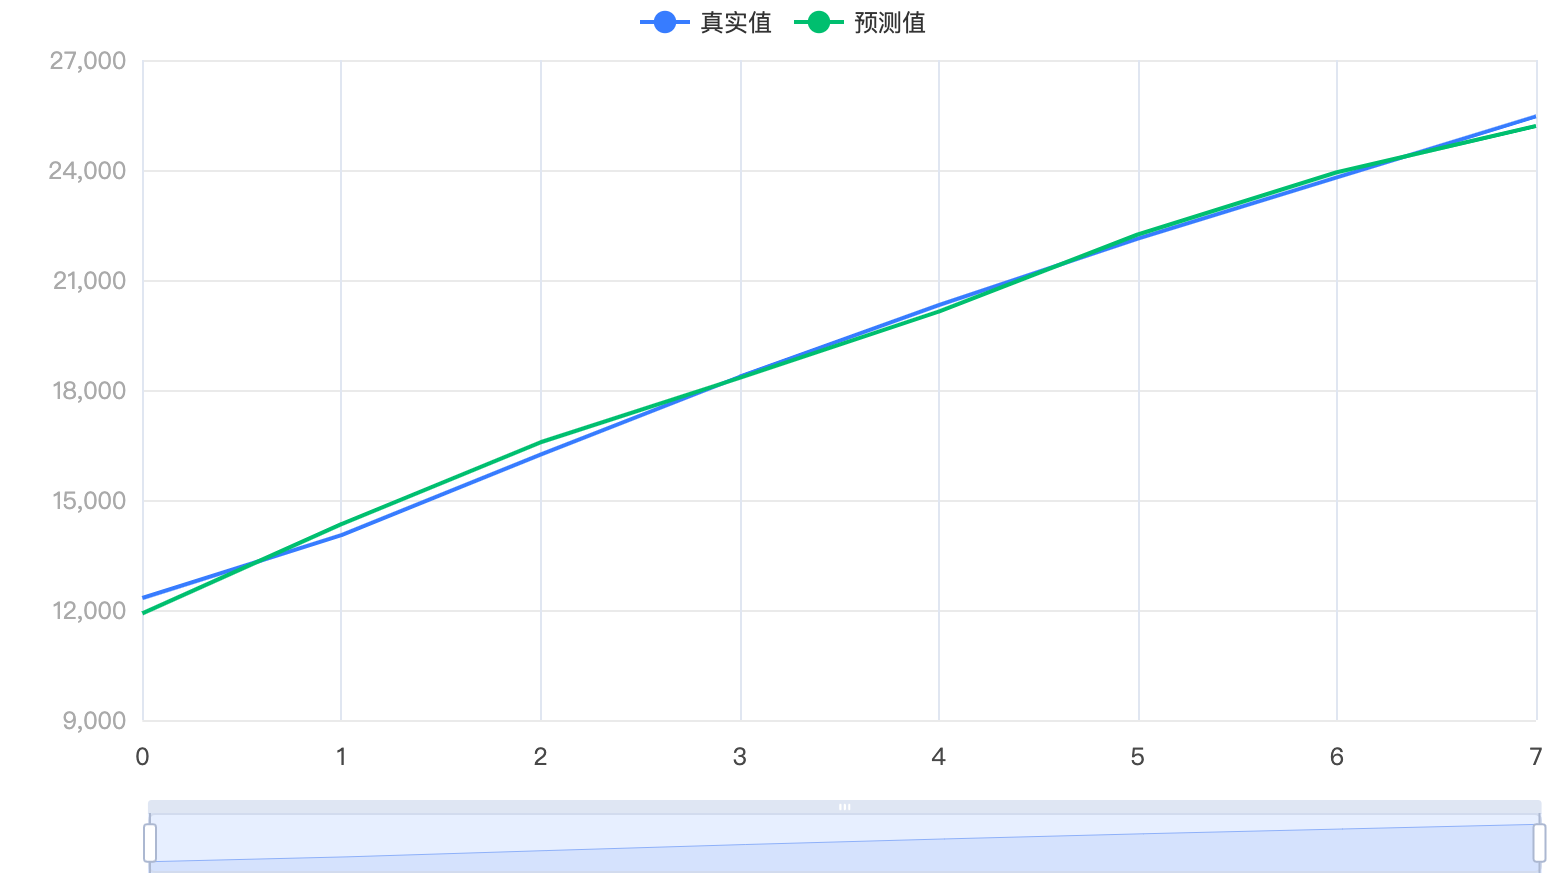
\includegraphics[width=0.8\textwidth]{pic/拟合效果图 (1).png}
  \caption{拟合效果图}
  \label{fig:拟合效果图}
\end{figure}

\begin{figure}[H]
  \centering
  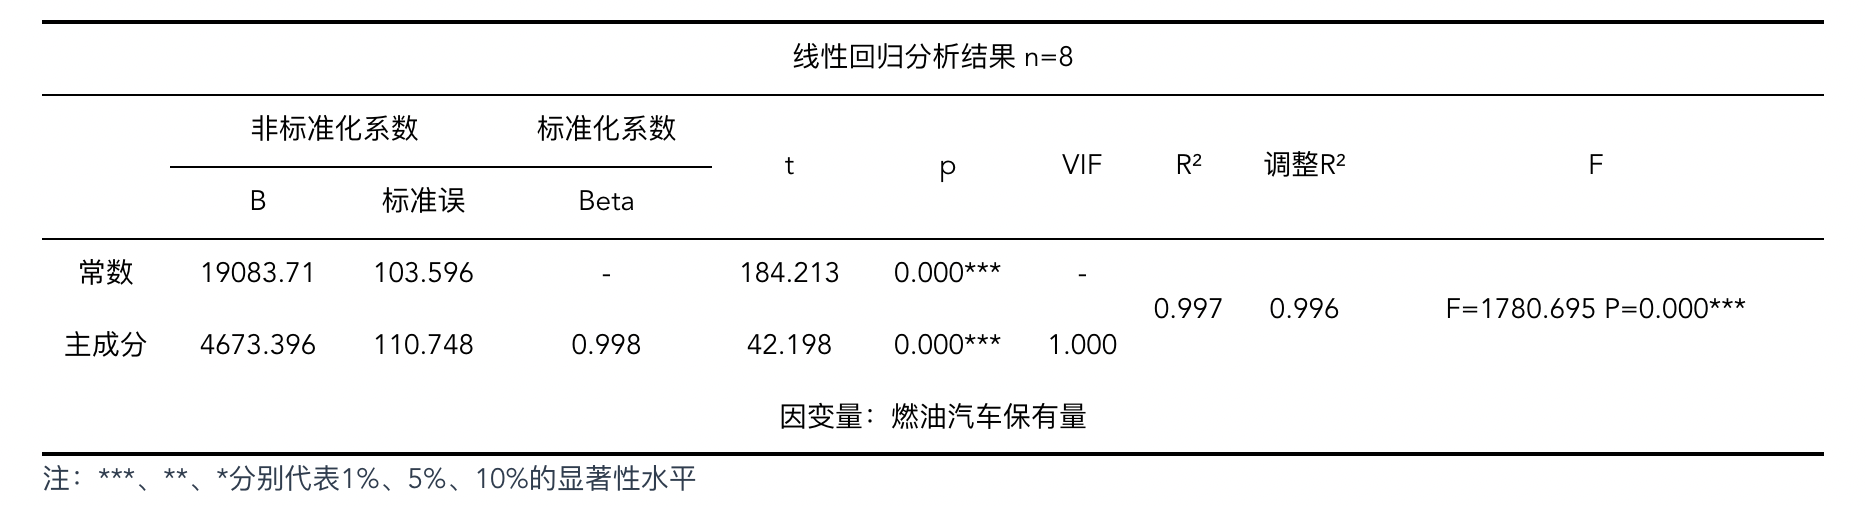
\includegraphics[width=\textwidth]{pic/截屏2022-05-19 下午5.30.59.png}
  \caption{线性回归分析结果}
  \label{fig:线性回归分析结果}
\end{figure}

燃油汽车保有量=19083.71+4673.396*主成分

% \begin{figure}[H]
%   \centering
%   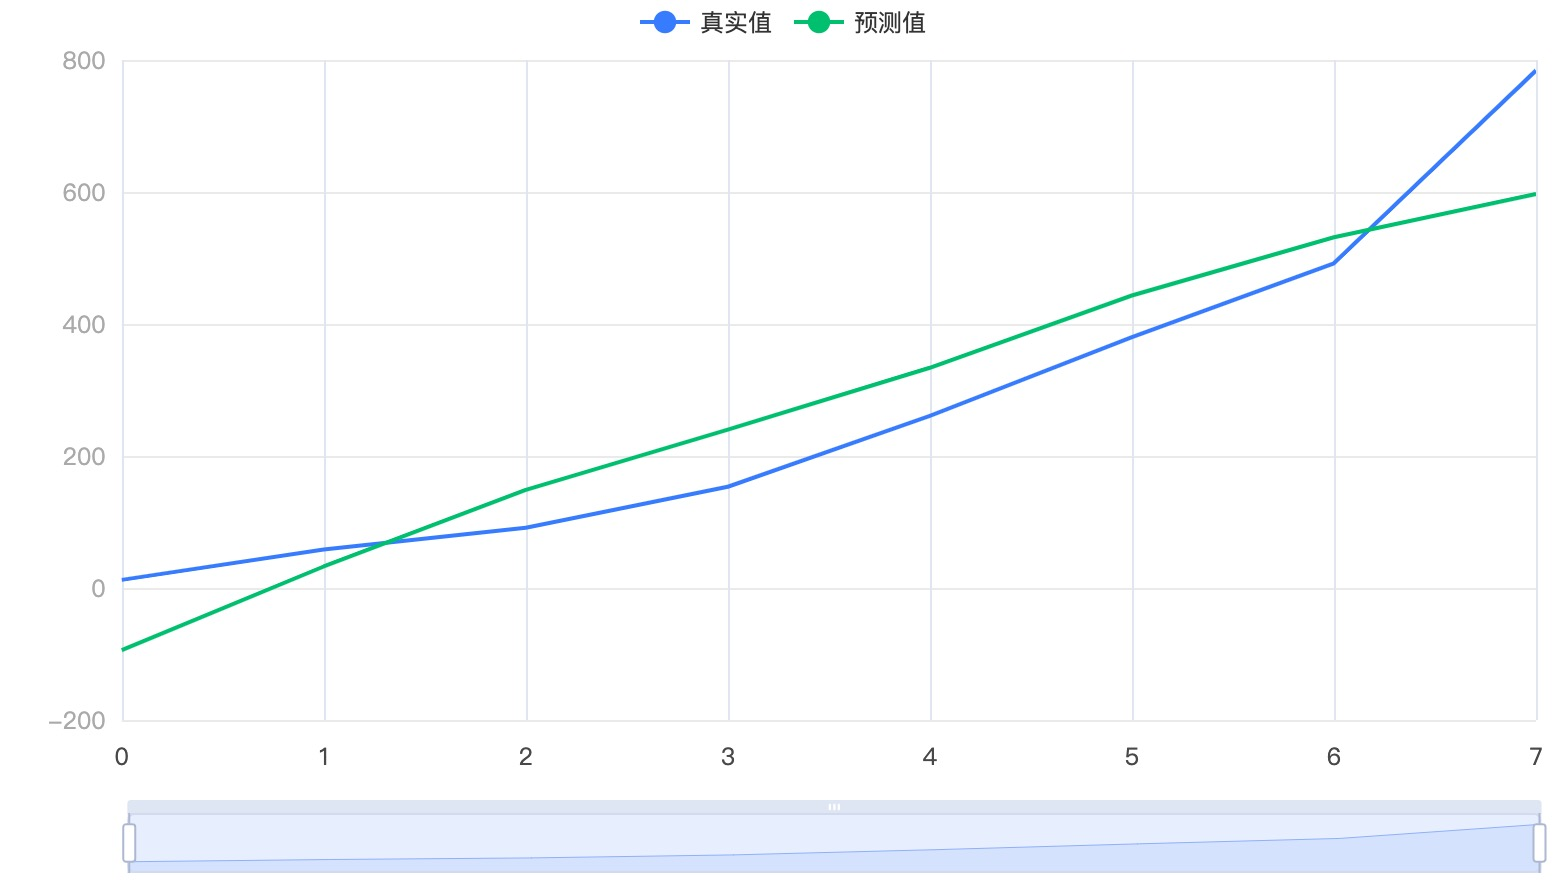
\includegraphics[width=0.8\textwidth]{pic/拟合效果图.png}
%   \caption{拟合效果图}
%   \label{fig:拟合效果图2}
% \end{figure}

\begin{figure}[H]
  \centering
  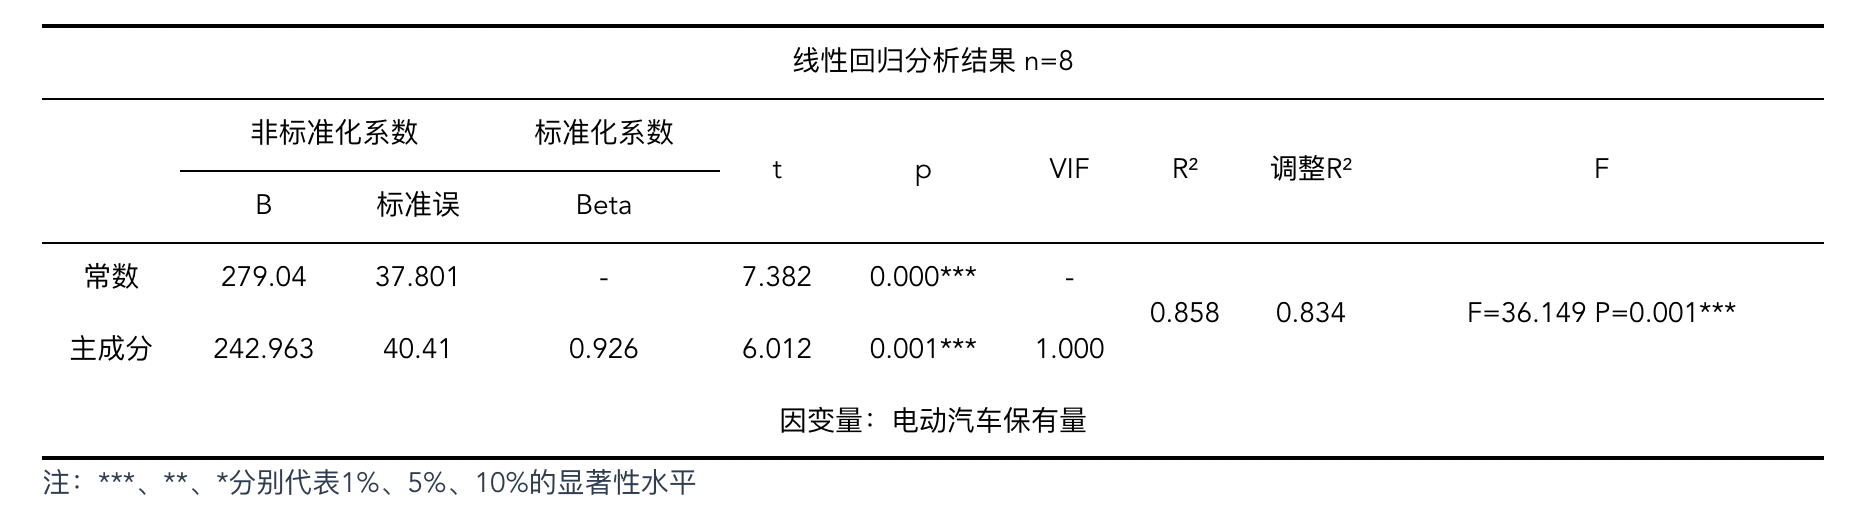
\includegraphics[width=\textwidth]{pic/截屏2022-05-19 下午5.29.26.png}
  \caption{线性回归分析结果}
  \label{fig:线性回归分析结果2}
\end{figure}

电动汽车保有量=279.04+242.963*主成分

以上回归分析结果中,从F检验的结果分析可以得到,显著性P值均为0.000***,水平上呈现显著性,
拒绝回归系数为0的原假设,
因此模型基本满足要求对于变量共线性表现,VIF全部小于10,模型没有多重共线性问题,
模型构建良好 。

\begin{equation}
  \sigma_1=\frac{4673.396}{19083.71}\approx0.24
\end{equation}

\begin{equation}
  \sigma_2= \frac{242.963}{279.04} \approx0.87
\end{equation}


\subsection{充电桩增长模型}
在初次建设充电桩时,我们时常无法一次性建设满足要求数量的充电桩。这时就需要根据人口、需求量、财富等因素得到优先级\(Pr_i=\alpha_1*Po_i+\alpha_2*q_i+\alpha_3*E\)逐步建立充电桩,(对应于p较小的时刻)。随着p的增长充电桩的数量得以逐步满足需求和冗余。

对于慢充来说,随着电池技术的发展,单次充电跨越时间T也会增长,同时随着经济增长,人均电动车数量也会同步增加,这两个因素的预测共同决定了\(q_i\)的发展。而对快充来说,随着科技的发展,充电速度则会提升(即平均服务时间减少),同时车辆的续航里程也会提升。我们依据电动车的增长模型所算得的数据再代入选址模型可以得到对充电桩选址的动态预测模型。



\section{模型求解}
\subsection{问题一的求解}
\subsubsection{充电桩选址}
我们从网上搜集到了L、\(F_k\)以及\(V_p\)数据,使用最短路径算法得到道路拓扑数据并将数据导入python(见附录\ref{code:load})。然后再从网络上得到杭州人口密度的热力图,通过matlab程序将两者结合(见附录\ref{code:heat2data}),如图\ref{fig:heat}所示:

\begin{figure}[H]
    \centering
    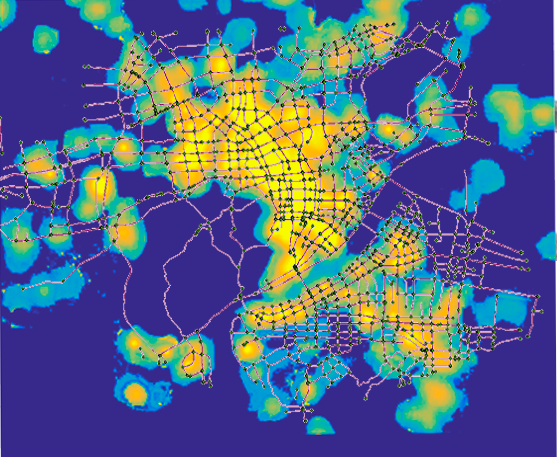
\includegraphics[width=0.8\textwidth]{pic/杭州道路-热力图.png}
    \caption{杭州道路-人口热力图}
    \label{fig:heat}
\end{figure}


接着我们再对线性规划方程(\ref{fun:优化lc})选用对的对偶单纯形(dual simplex)算法(见附录\ref{code:优化})求解得到结果如图所示。

\subsubsection{充电桩未来发展趋势}

\textbf{人口预测}:

通过对近年人口预测论文的阅读,我们发现主流的人口预测模型为灰色模型。因此我们在SPSSPRO中使用灰色预测模型GM(1,1)通过1964---2021年我国总人口数对未来十年我国总人口数。

得到灰色模型构建结果如下:

\begin{table}[H]
  \centering
  \begin{tabularx}{0.9\textwidth}{XXX}
  \toprule
  发展系数a & 灰色作用量b & 后验差比C值 \\
  \midrule
  -0.011 & 554.104 & 0.035 \\
  \bottomrule
  \end{tabularx}
  \caption{灰色模型构建}
  \label{tab:grey}
\end{table}

从上表分析可以得到,后验差比值为0.035,模型精度高。

模型拟合预测图:
\begin{figure}[H]
  \centering
  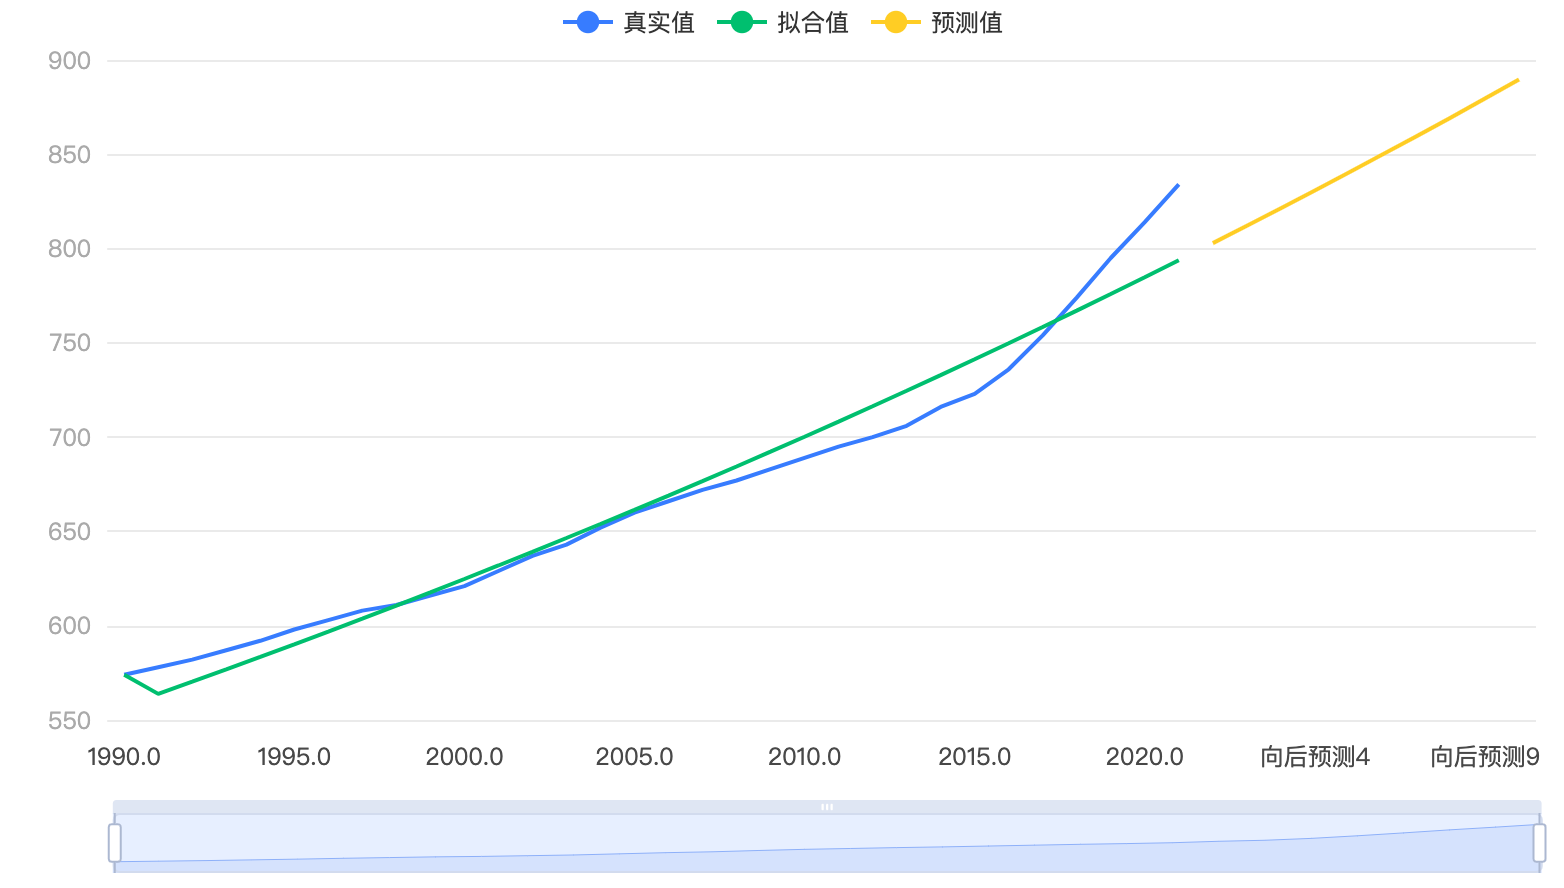
\includegraphics[width=0.8\textwidth]{pic/模型拟合预测图.png}
  \caption{模型拟合预测图}
  \label{fig:模型拟合预测图}
\end{figure}



预测得2027年杭州总人口数为840.3万人,2032年杭州总人口数为889.6万人。

\textbf{经济预测:}

我们以1990-2021年杭州市人均GDP作为杭州市经济的衡量指标。我们在SPSSPRO中使用ARIMA模型对未来十年杭州市人均GDP做预测。

\begin{table}[H]
  \centering
  \begin{tabularx}{0.9\textwidth}{llXXXXXX}
  \toprule
  \multicolumn{8}{c}{ADF检验表}\\
  \midrule
  变量 & 差分阶数 & t & p & AIC & 临界值 & & \\
  1\% & 5\% & 10\% & & & & & \\
  人均gdp & 0 & 0.239 & 0.974 & 452.928 & -3.661 & -2.961 & -2.619 \\
  1 & -6.73 & 0.000*** & 451.419 & -3.67 & -2.964 & -2.621 & \\
  2 & -2.027 & 0.275 & 435.42 & -3.809 & -3.022 & -2.651 & \\
  \bottomrule
  \end{tabularx}
  \caption{ADF检验表}
  \label{tab:ADF}
\end{table}

在差分为0阶、2阶时,显著性P值为0.974、0.275,水平上不呈现显著性,不能拒绝原假设,该序列均为不平稳的时间序列。
在差分为1阶时,显著性P值为0.000***,水平上呈现显著性,拒绝原假设,该序列为平稳的时间序列。

1阶差分时序图:

\begin{figure}[H]
  \centering
  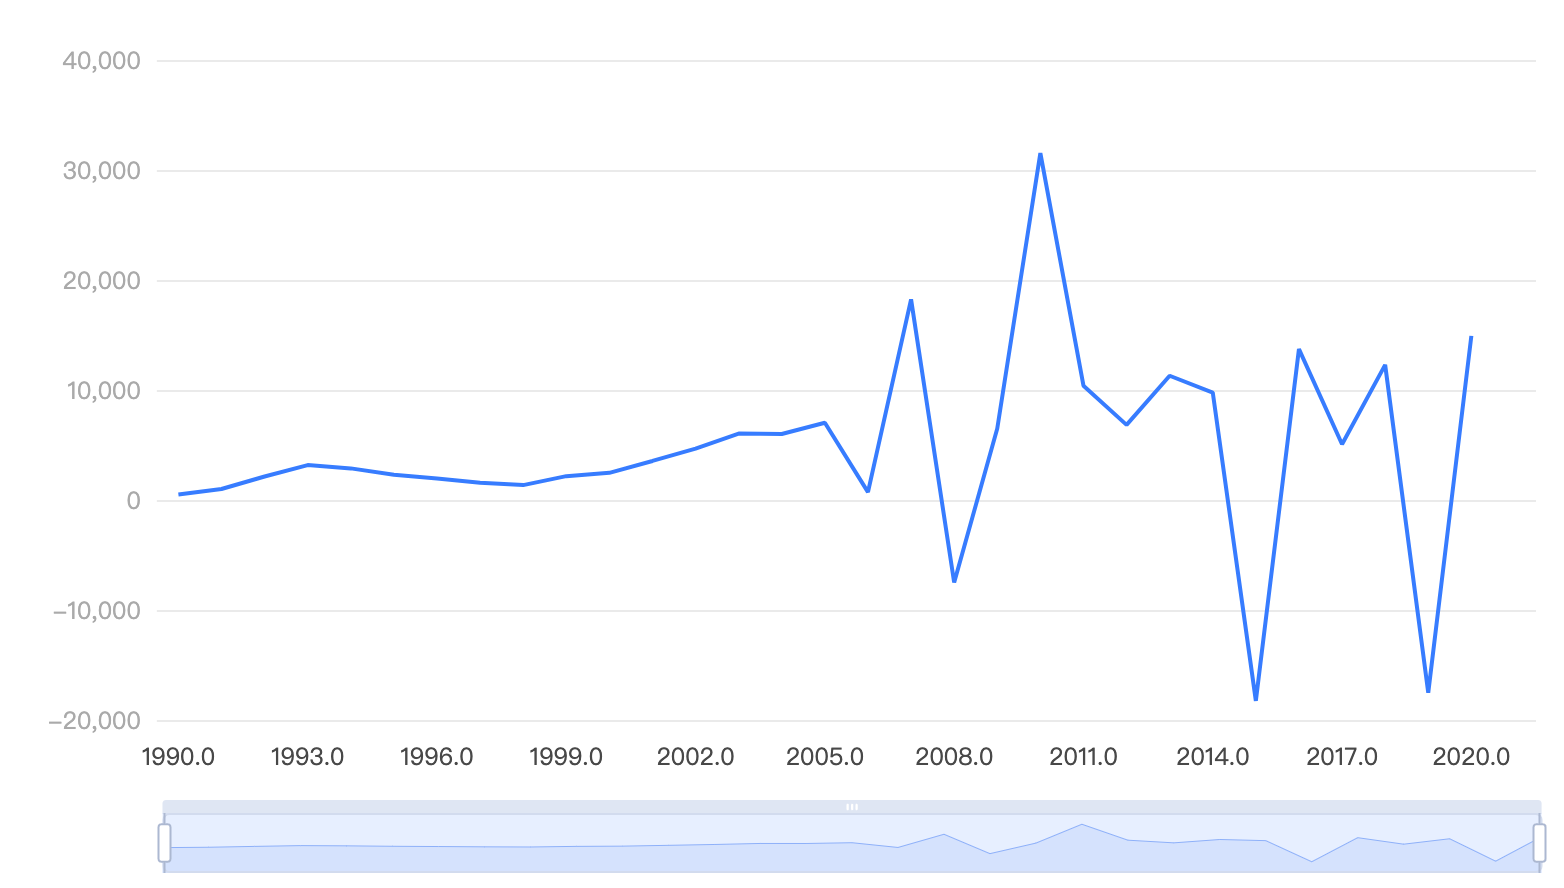
\includegraphics[width=0.8\textwidth]{pic/最佳差分序列图.png}
  \caption{最佳差分序列图}
  \label{fig:最佳差分序列图}
\end{figure}



最终差分数据自相关图(ACF):

\begin{figure}[H]
  \centering
  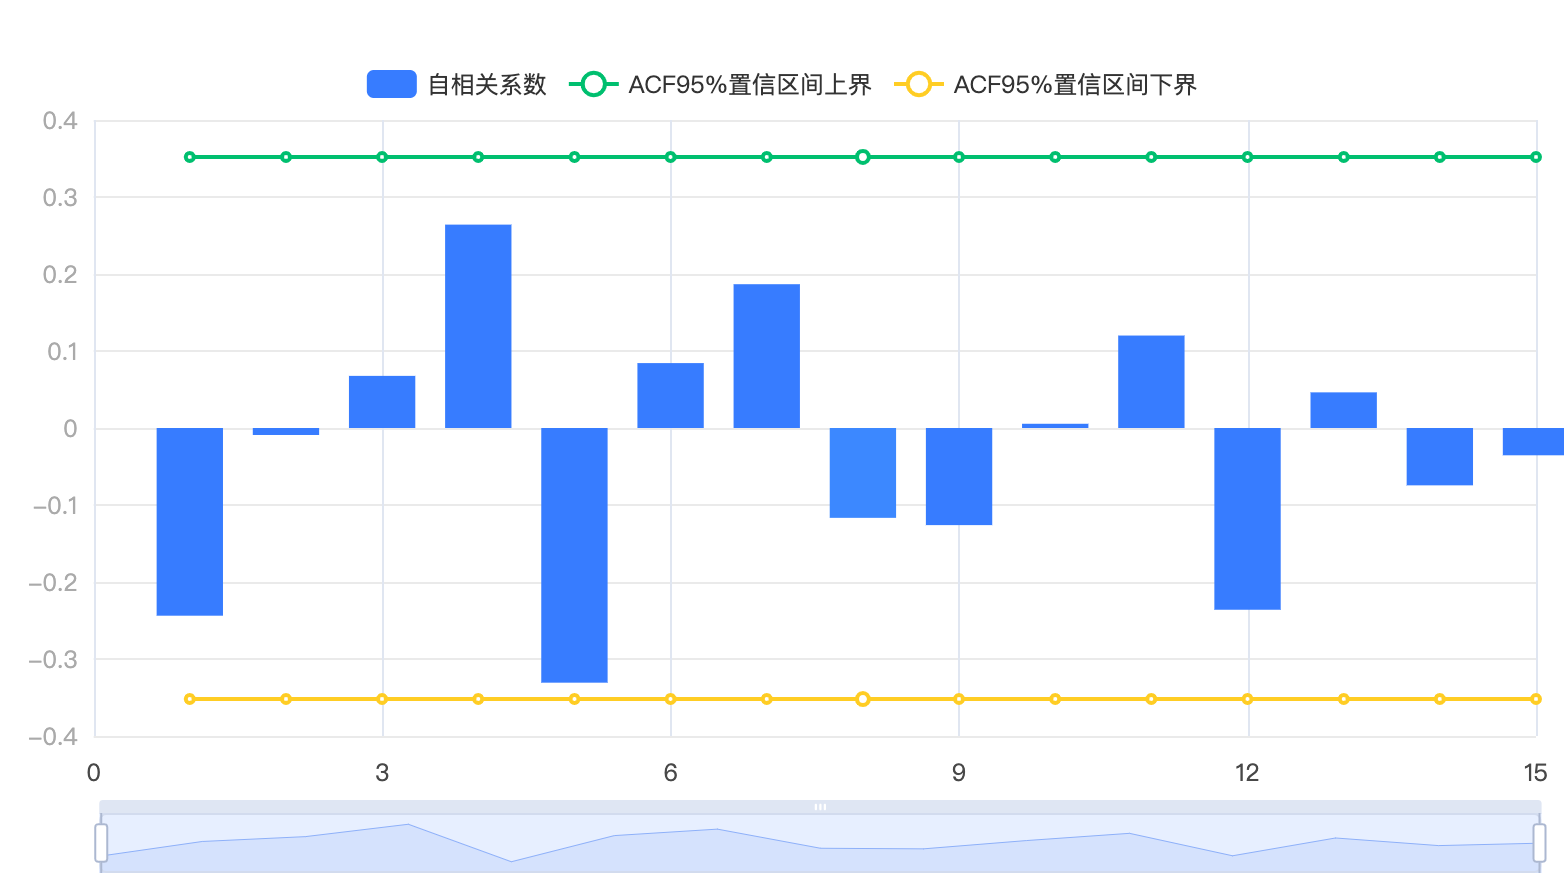
\includegraphics[width=0.8\textwidth]{pic/最终差分数据自相关图(ACF) (1).png}
  \caption{最终差分数据自相关图(ACF)}
  \label{fig:ACF}
\end{figure}


ARIMA模型(0,1,0)检验表如下,得到模型结果为ARIMA模型(0,1,0)检验表,从Q统计量结果分析可以得到:Q6在水平上不呈现显著性,不能拒绝模型的残差为白噪声序列的假设,同时模型的拟合优度R2为0.968,模型表现优秀,模型基本满足要求。

\begin{table}[H]
  \centering
  \begin{tabularx}{0.9\textwidth}{XXX}
  \toprule
  & ARIMA模型(0,1,0)检验表 & \\
  \midrule
  项 & 符号 & 值 \\
  & Df Residuals & 30 \\
  样本数量 & N & 32 \\
  Q统计量 & Q6(p值) & 2.026(0.155) \\
  Q12(p值) & 9.435(0.151) & \\
  Q18(p值) & 16.005(0.191) & \\
  Q24(p值) & 16.657(0.547) & \\
  Q30(p值) & 17.06(0.846) & \\
  信息准则 & AIC & 656.864 \\
  BIC & 659.732 & \\
  拟合优度 & R² & 0.968 \\
  \bottomrule
  \end{tabularx}
  \caption{ARIMA模型(0,1,0)检验表}
  \label{tab:arima}
\end{table}

得到时间序列图:

\begin{figure}[H]
  \centering
  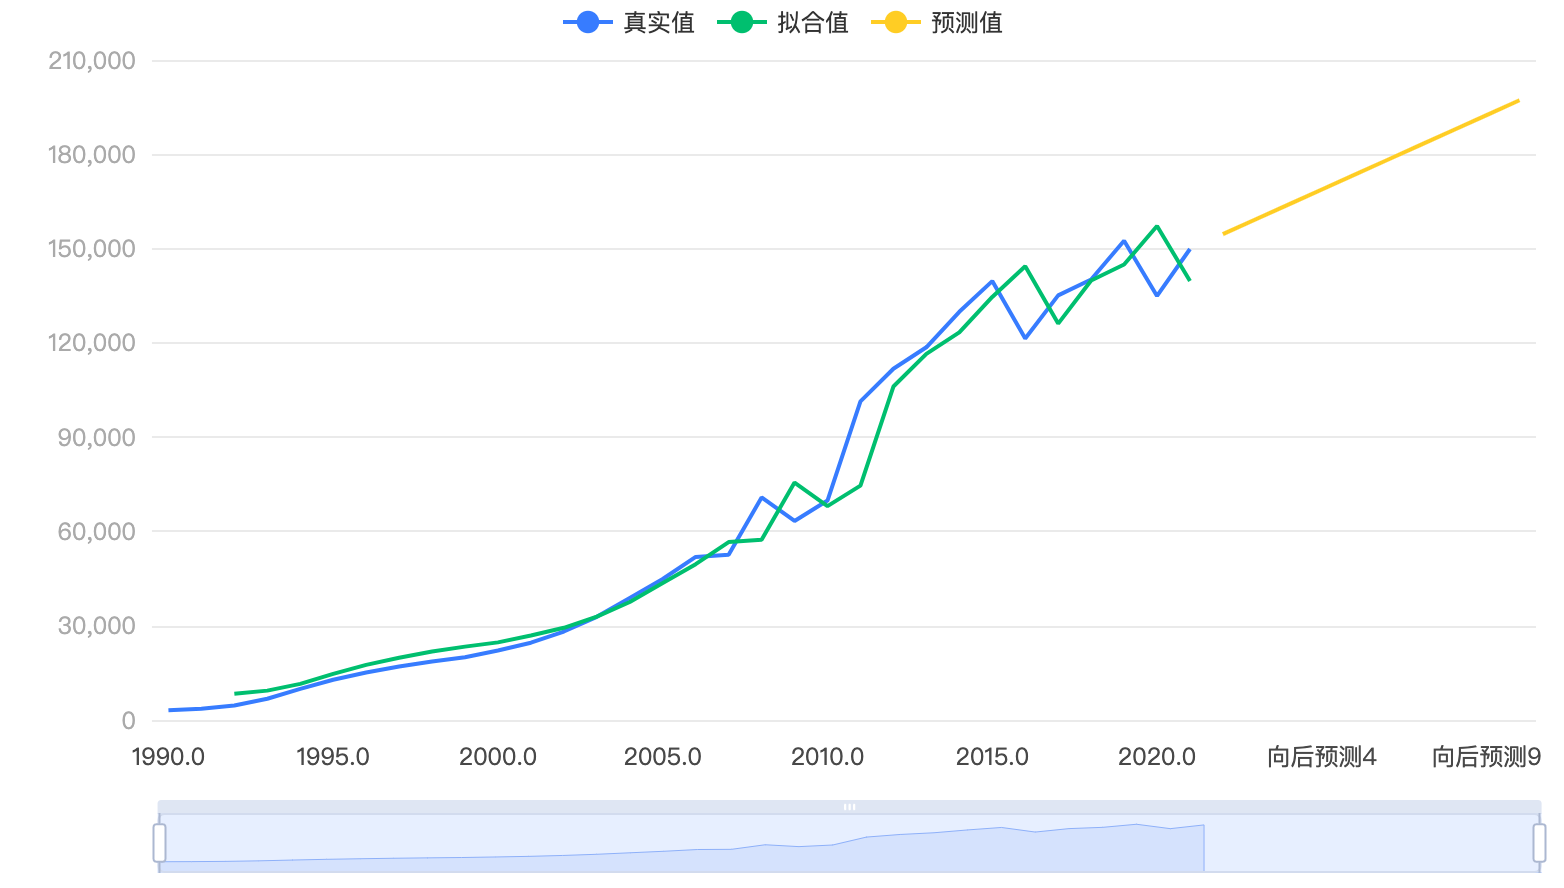
\includegraphics[width=0.8\textwidth]{pic/时间序列图.png}
  \caption{时间序列图}
  \label{fig:时间序列图}
\end{figure}



预测2027年杭州市人均GDP为173526人民币,2032年杭州市人均GDP为197195万元。


根据我们对于电动车增长的预测模型,代入重新计算了充电桩的选址,可以得到以下充电桩发展图:

首先是初次建立充电桩时的逐步选址图,以下分别列出了p只有当前需求25\%、50\%、75\%和100\%时的优先级选址:



接着是随着电动车发展而导致的充电桩选址建设预测(假定政府会根据预测提前开始建造充电设施,因此无需关心优先级),以下是n年后、2n年后的充电桩选址:


\subsection{问题二的求解}
\subsubsection{模型的求解}

我们使用matlab对该生物种群相互竞争模型进行求解,得到如下结果:

\begin{figure}[H]
  \centering
  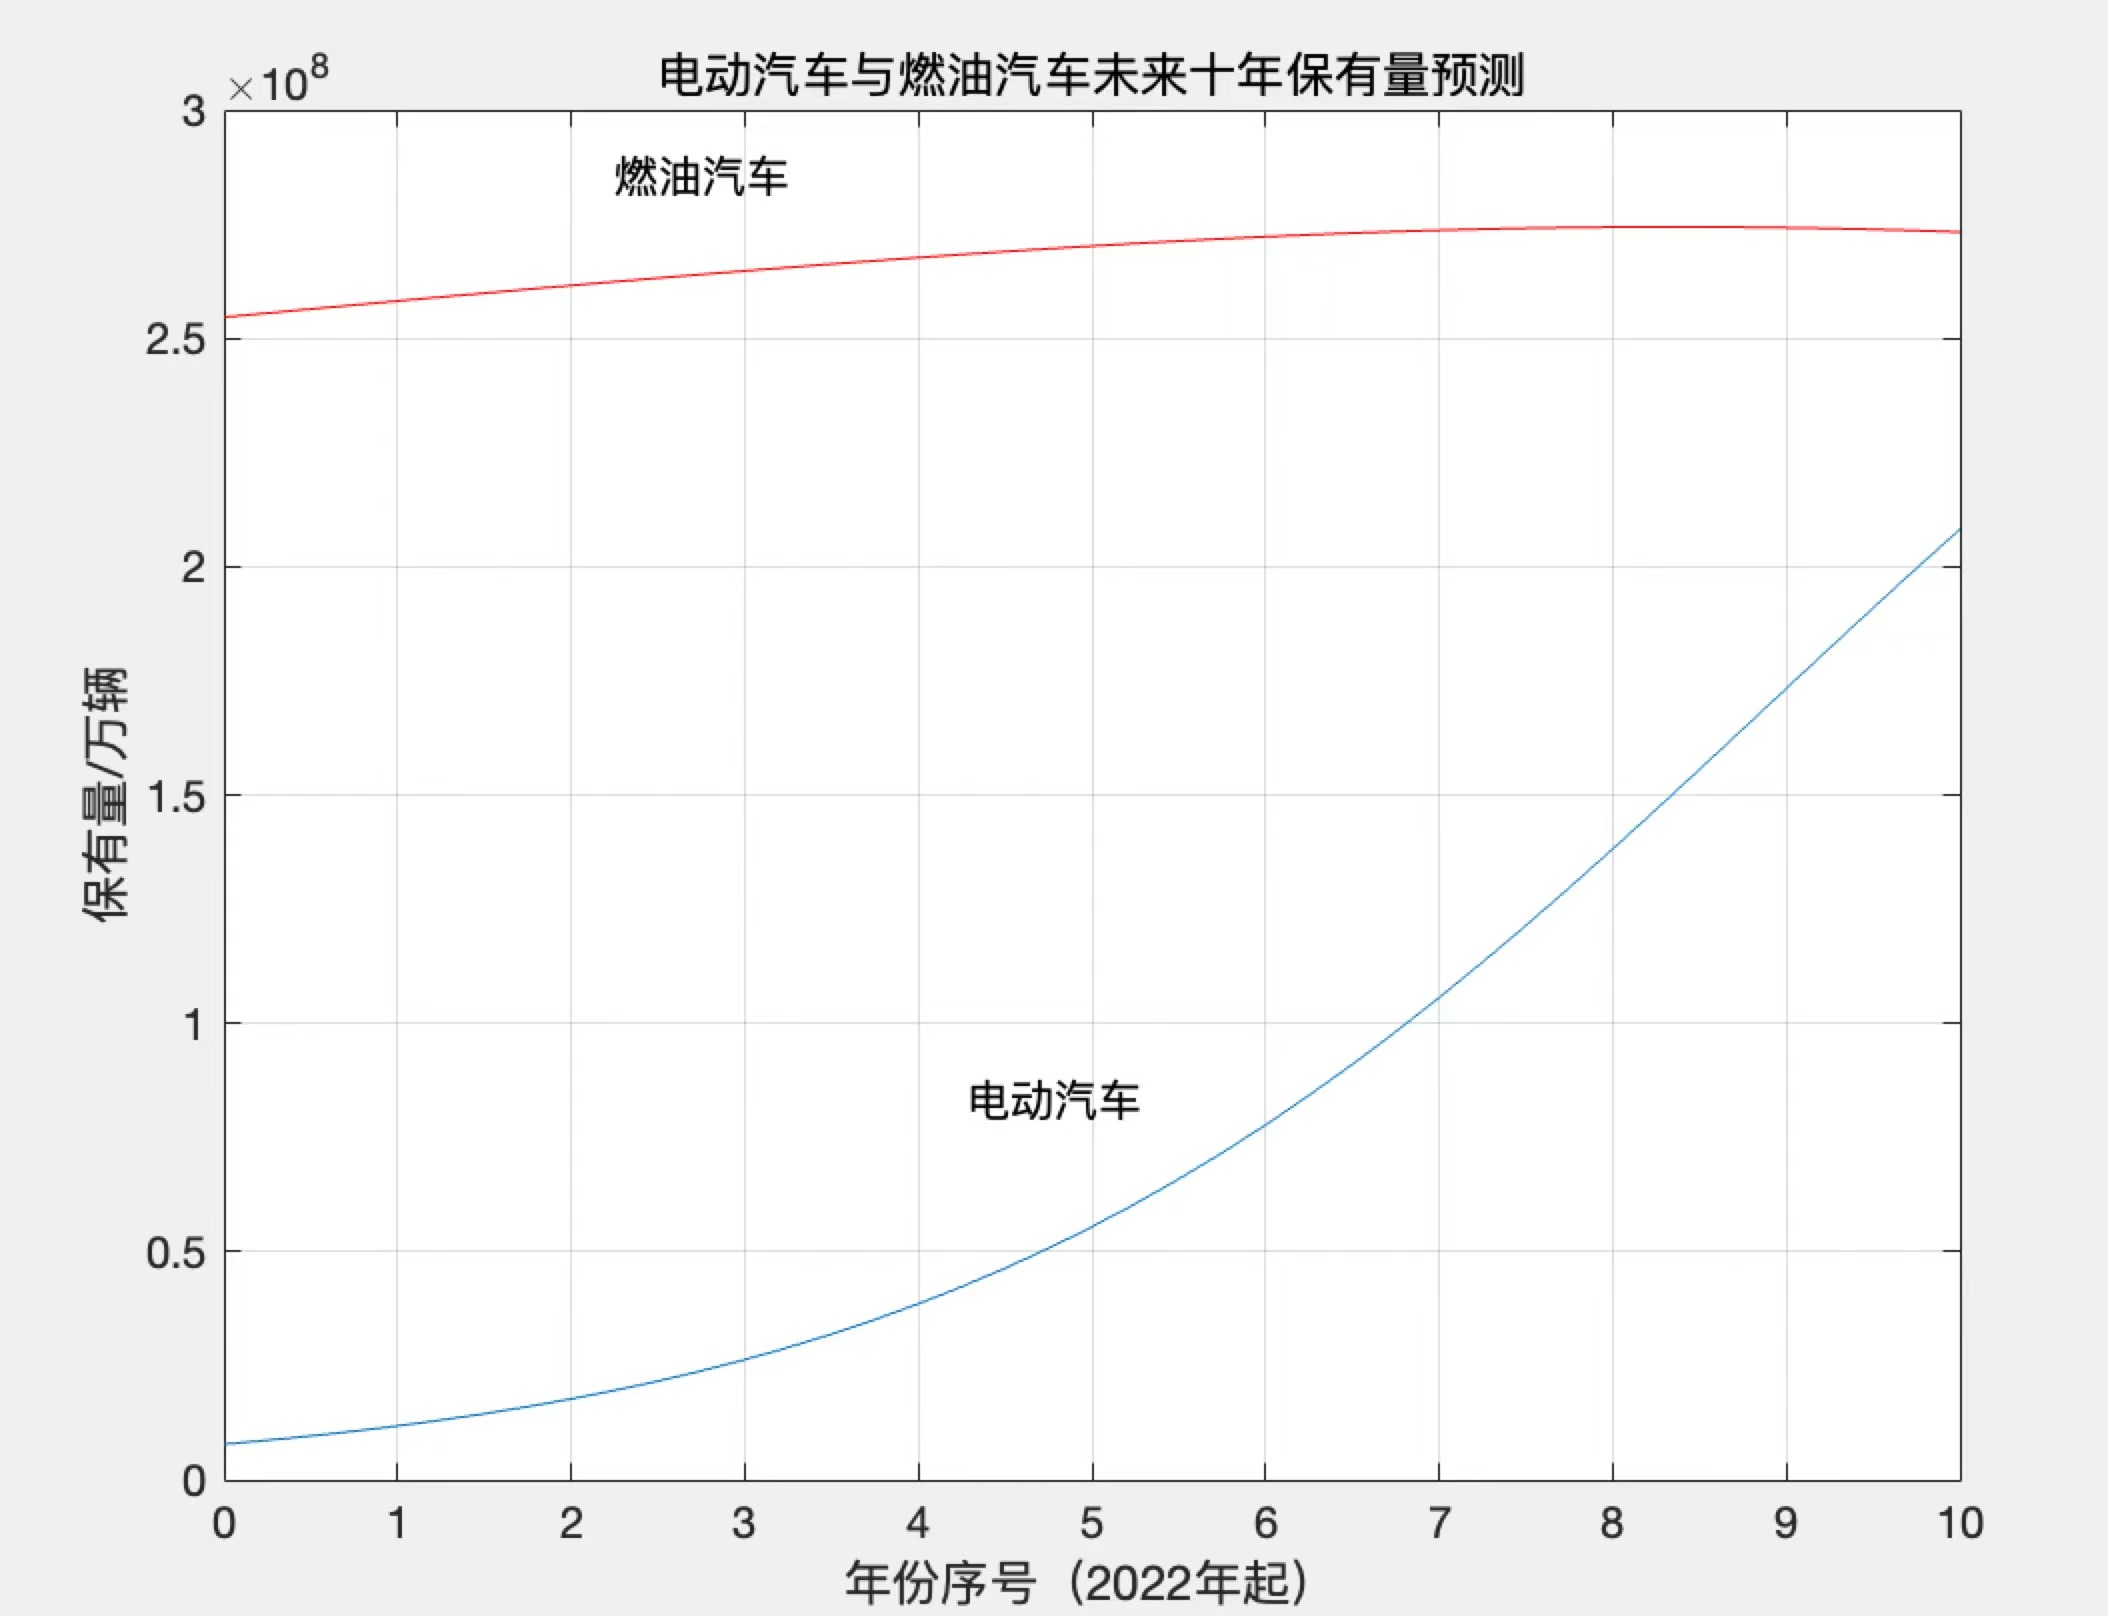
\includegraphics[width=\textwidth]{pic/911652953505_.pic.jpg}
  \caption{电动汽车与燃油汽车未来十年保有量预测}
  \label{fig:电动汽车与燃油汽车未来十年保有量预测}
\end{figure}

根据最新统计数据,2022年第一季度电动汽车保有量为891.5万辆,与我们预测的结果873.9万辆基本接近。




\section{模型评价}
\subsection{敏感性分析}
\subsection{优点}
\subsection{不足}
\subsection{展望}


\begin{thebibliography}{99}
    \bibitem{cite:统计年鉴}中华人民共和国统计局.中国统计年鉴(2021)[M].北京:中国统计出版社,2022.
    \bibitem{cite:预测报告}
\end{thebibliography}
\newpage
\section{附录}
\appendix
\section{代码}
\subsection{导入数据到python}
\label{code:load}
\lstset{language=python}
\lstset{
    numbers=left, 
    numberstyle= \tiny, 
    keywordstyle= \color{ blue!70},
    commentstyle= \color{red!50!green!50!blue!50}, 
    frame=shadowbox, % 阴影效果
    rulesepcolor= \color{ red!20!green!20!blue!20} ,
    escapeinside=``, % 英文分号中可写入中文
    xleftmargin=2em, aboveskip=1em,
    framexleftmargin=2em
}

\lstinputlisting[caption={\bf load.py}]{code/load.py}
\lstinputlisting[caption={\bf loadxy.py},language=Python,]{code/loadxy.py}

\subsection{转化热力图的matlab代码}
\label{code:heat2data}
\lstinputlisting[caption={\bf heat2data.m},language=Matlab,style={Matlab-editor}]{code/heat2data.m}

\subsection{求解优化问题的python代码}
\label{code:优化}

\end{document}
